% ============================================================
% D68 — The Pulsation as a Bipartition: Complete Classification of
%       C1-Admissible Dynamical Laws, and a Singleton Obstruction
%       Theorem for Frustration-Based Selection
%
% Author  : Cédric Laubscher
% Corpus  : PDL Document Series, D68
% Version : 4 (adds Erratum 3 in D43: the 204+228 bridge that does not
%           close; the identity 101 = n_K + (Delta n + 1)^2 resolving a
%           long-standing corpus discrepancy; and the hierarchical
%           reading that legitimises c = 3. See Section 11.2.)
% Version : 3 (errata verified against the D46 source and strengthened;
%           OP-D68-7 added recording the divergence between D46's
%           definition of the pulsation and the one derived here;
%           the earlier claim that the errata do not propagate is
%           WITHDRAWN, see Section 11.1)
%
% Depends : D01 (10.5281/zenodo.18462686)
%           D02 (10.5281/zenodo.18463130)
%           D08 (10.5281/zenodo.18664995)
%           D33 (10.5281/zenodo.19307249)
%           D46 (10.5281/zenodo.19956932)
%           D60 (10.5281/zenodo.20639684)
%           D61 (10.5281/zenodo.20645713)
%           D66 (10.5281/zenodo.21351177)
%           D67 (10.5281/zenodo.21382362)
%
% CORRECTION LOG (see Section 11 for the full account):
%   (C1-err) D46, Table 1: the eight coherent configurations of K_4
%            are listed as four pairs {s, -s}. The four entries of
%            the form s^(2) = -s^(1) are NOT coherent. The correct
%            decomposition is 1 + 3 + 4 (D60). ERRATUM.
%   (C1b-err) D46, Table 1: only FOUR of the EIGHT coherent
%            configurations are listed; the four listed form a Klein
%            subgroup (cuts empty, {3}, {2}, {0,1}). ERRATUM.
%   (C2-err) D46, Lemma "Global sign flip preserves triangular
%            coherence": the heading and statement contradict the
%            proof printed beneath them. Corrected to "reverses".
%            D46's following remark shows the author was aware of
%            the difficulty; only the formal statement is wrong.
%   (C6-err) D43: "204 + 228 = 329" does not close (204+228=432). The
%            sentence is a narrative bridge, not the derivation; the
%            theorem gives n_K(1+c) + 25 = 304 + 25 = 329 exactly.
%            ERRATUM.
%   (C7-res) The discrepancy E_sea - R_sea = 10188 - 10087 = 101, and
%            the gap 329 - 228 = 101, are the same number, and
%            101 = n_K + (Delta n + 1)^2 = 76 + 25. RESOLVED.
%   (C8-cla) c = 3 is legitimate under the hierarchical reading: each
%            entity of a valence core IS a K_4 closure at the level
%            below; there are no K_4 sub-blocks inside K_24 or K_28.
%            CLARIFICATION, no result changed.
%   (C5-div) D46 defines the pulsation as the global edge reversal
%            s -> -s; this document derives it as a switching.
%            NOT an erratum: a divergence of definition, recorded
%            as OP-D68-7 and not adjudicated here.
%   (C3-cla) D60 describes the discrepancy with D46 as a "potential
%            ambiguity". It is an error, not an ambiguity.
%            CLARIFICATION, no mathematical consequence for D60.
%   (C4-cla) D60's orbit decomposition 1+3+4 is here re-derived as a
%            classification by cut size, and verified configuration
%            by configuration in Section 10. No change to D60.
% ============================================================

\documentclass[11pt,a4paper]{article}
\usepackage[utf8]{inputenc}
\usepackage[T1]{fontenc}
\usepackage[english]{babel}
\usepackage{lmodern}
\usepackage{microtype}
\usepackage{amsmath,amssymb,amsthm}
\usepackage{mathtools}
\usepackage[colorlinks=true,linkcolor=blue,citecolor=blue,urlcolor=blue]{hyperref}
\usepackage[numbers]{natbib}
\usepackage[most]{tcolorbox}
\usepackage{geometry}
\geometry{margin=2.5cm}
\usepackage{booktabs}
\usepackage{longtable}
\usepackage{array}
\usepackage{xcolor}
\usepackage{tikz}
\usetikzlibrary{arrows.meta,positioning,fit,backgrounds}

\pdfstringdefDisableCommands{%
  \def\ensuremath{}%
  \def\mathrm#1{#1}%
  \def\mathcal#1{#1}%
}

% ---- Theorem environments ----
\newtheorem{theorem}{Theorem}[section]
\newtheorem{lemma}[theorem]{Lemma}
\newtheorem{corollary}[theorem]{Corollary}
\newtheorem{proposition}[theorem]{Proposition}
\newtheorem{definition}[theorem]{Definition}
\newtheorem{remark}[theorem]{Remark}
\newtheorem{negresult}[theorem]{Negative Result}
\newtheorem{openproblem}{Open Problem}
\newtheorem{erratum}{Erratum}

% ---- PDL macros ----
\newcommand{\PDL}{\textsc{pdl}}
\newcommand{\Kfour}{K_4}
\newcommand{\Kn}{K_n}
\newcommand{\Coh}{\mathrm{Coh}}
\newcommand{\Aut}{\mathrm{Aut}}
\newcommand{\cross}{\mathrm{cross}}
\newcommand{\mono}{\mathrm{mono}}
\newcommand{\dtg}{d}
\newcommand{\etaL}{\eta_L}

\definecolor{proofblue}{RGB}{0,70,150}
\definecolor{negred}{RGB}{150,30,30}

\newtcolorbox{theorembox}[1][]{colback=blue!5,colframe=blue!60!black,fonttitle=\bfseries,title=#1}
\newtcolorbox{negbox}[1][]{colback=red!5,colframe=red!60!black,fonttitle=\bfseries,title=#1}
\newtcolorbox{openprobbox}[1][]{colback=orange!8,colframe=orange!70!black,fonttitle=\bfseries,title=#1}
\newtcolorbox{errbox}[1][]{colback=gray!8,colframe=gray!60!black,fonttitle=\bfseries,title=#1}

\title{\textbf{The Pulsation as a Bipartition}\texorpdfstring{\\[4pt]\large Complete Classification of C1-Admissible Dynamical Laws, and a Singleton Obstruction Theorem for Frustration-Based Selection}{: Complete Classification of C1-Admissible Dynamical Laws, and a Singleton Obstruction Theorem for Frustration-Based Selection}\\[6pt]
{\large PDL Document D68}}

\author{C\'edric Laubscher\\[4pt]
\small Independent Researcher, Switzerland\\
\small \href{https://cedriclaubscher.ch}{cedriclaubscher.ch}}

\date{August 2026}

\begin{document}
\maketitle

\begin{abstract}
The founding question of the \PDL\ programme --- what distinguishes something that exists from something that does not --- is answered in axiom C1 by the postulate of a repeatable, non-trivial binary alternation. The corpus has never argued for C1; it has only assumed it. This document supplies the missing argument, quarantined in an appendix as motivation rather than proof, and then determines exhaustively what C1 can and cannot mean.

Three results are established as unconditional theorems of C1--C4. First, a C2-admissible sign configuration on a complete signed graph is exactly a bipartition of its vertices, and the pulsation is exactly a switching by a fixed vertex subset: an involution, hence a two-cycle by construction. Second, the pulsation laws compatible with C1 are completely classified. On $n$ entities there are exactly $2(2^n-2)$ admissible laws, falling into exactly two families and no third, and generating exactly $2^{n-1}-1$ distinct relational dynamics --- in bijection with the non-trivial coherent configurations. In particular, a strictly universal simultaneous inversion of every entity is the trivial element: it is not incoherent but empty, being the exact gauge redundancy already identified as the $\mathrm{U}(1)$ global phase in D46. What survives is a partition of the entities into two phase classes, all entities sharing one period and differing only by a binary offset, each changing state exactly once per relational cycle. Third, the set of frustrated triangles is pointwise invariant under every switching, so the classification is independent of frustration and is not a property of the balanced idealisation.

Two negative results follow, both first-class. C4 is blind to the pulsation: the frustration count is identical across all $2^{n-1}-1$ candidate bipartitions, so no minimisation of leakage can select one. And the natural refinement that does select --- minimising the frustration carried across the pulsating boundary --- always selects a cut of size one, that is, a single privileged entity, which is inadmissible in a relational theory. This last statement is proved here as a theorem for all $n$ and all cut sizes; the proof turns entirely on the two-graph parity condition, and is reproduced exactly on the extremal family. A corollary excludes every functional built from frustration and group size alike.

Section~\ref{sec:worked} carries every object of the paper through explicitly on $\Kfour$, configuration by configuration, so that the results can be checked by hand before any script is run. Two errata in D46 are recorded and corrected against the source, and a divergence between D46's definition of the pulsation and the one derived here is recorded as an open problem. A third erratum, in D43, is also recorded: an arithmetic bridge that does not close, whose correction resolves a discrepancy of $101$ that the corpus has carried unexplained, by exhibiting it as $n_K+(\Delta n+1)^2=76+25$. Five verification scripts, exhaustive up to $n=7$, are deposited with this document under the same \textsc{doi}, with their expected outputs tabulated in Section~\ref{sec:scripts}.
\end{abstract}

\clearpage
\tableofcontents
\newpage

% ============================================================
\section{Introduction and position in the causal chain}
\label{sec:intro}
% ============================================================

\subsection{The founding question, and what the corpus never said}

The \PDL\ programme derives physical structure from four axioms on finite signed graphs, without presupposing spacetime, particles or fields~\citep{D01,D02}. The first of these axioms, C1, states that existence is instantiated as a repeatable, non-trivial alternation between two discrete states, independent of any pre-existing temporal metric.

C1 has been used, in one form or another, in nearly every subsequent document of the corpus. It has never been argued for. It is posited, and the programme proceeds. This is a genuine gap in a programme whose stated ambition is to derive rather than to assume.

The argument the axiom always had, and never carried in writing, is given in Appendix~\ref{app:ontology}. It is placed there deliberately. It is an argument about indiscernibility, not a proof, and it does not have the status of anything else in this document; a reader who rejects it entirely loses nothing of Sections~\ref{sec:prereq} to~\ref{sec:worked}, which depend on C1 as stated and not on any motivation for it. It is included because a programme that asks why there is something rather than nothing should say, somewhere, why its first axiom takes the form it does.

\subsection{The question this document answers}

The intuitive reading of C1 is that every entity of the universe changes state at each cycle, and that the global pattern therefore inverts at each pulsation. If all entities are identical in nature, as the programme maintains, this reading is the natural one.

It is wrong, and it is wrong in an instructive way. Section~\ref{sec:trivial} proves that a strictly universal simultaneous inversion is the identity on the relational state: it changes nothing that any measurement could detect. It is not incoherent; it is empty, and it is exactly the global $\mathrm{U}(1)$ phase already derived in D46~\citep{D46}, restated in combinatorial rather than complex-analytic terms.

What replaces it preserves the intuition entirely. Section~\ref{sec:classification} classifies every pulsation law compatible with C1, exhaustively, and the surviving picture is this: all entities share one and the same period, all are identical in nature, and they are distinguished only by a binary phase offset that partitions them into two classes. Each entity changes state exactly once per relational cycle. The vertex pattern does invert completely, as the intuition demands --- but the full inversion takes two logical steps rather than one, and the completely inverted state is relationally identical to the starting state. What is observable is the intermediate state. This is the combinatorial shadow of $T^2=-I_2$ (D33~\citep{D33}, lifted in D46).

Sections~\ref{sec:frustration} to~\ref{sec:obstruction} then ask whether the axioms determine \emph{which} bipartition. They do not, and the reason is sharp enough to be proved.

\subsection{How to read this document}

Figure~\ref{fig:chain} shows the logical architecture in full. Each axiom contributes one structural fact, and the four facts compose into a classification and then into two obstructions.

A reader who prefers concrete objects to abstract ones may go directly to Section~\ref{sec:worked}, which carries every construction of this paper through explicitly on $\Kfour$: the eight coherent configurations written out, their identification with the eight bipartitions, the correspondence with the orbit decomposition of D60 checked configuration by configuration, one pulsation followed step by step, and one frustrated example in which the crossing functional is evaluated on every cut. Nothing in Section~\ref{sec:worked} requires a computer. It is intended to make the general statements checkable by hand before any script is run.

\begin{figure}[htbp]
\centering
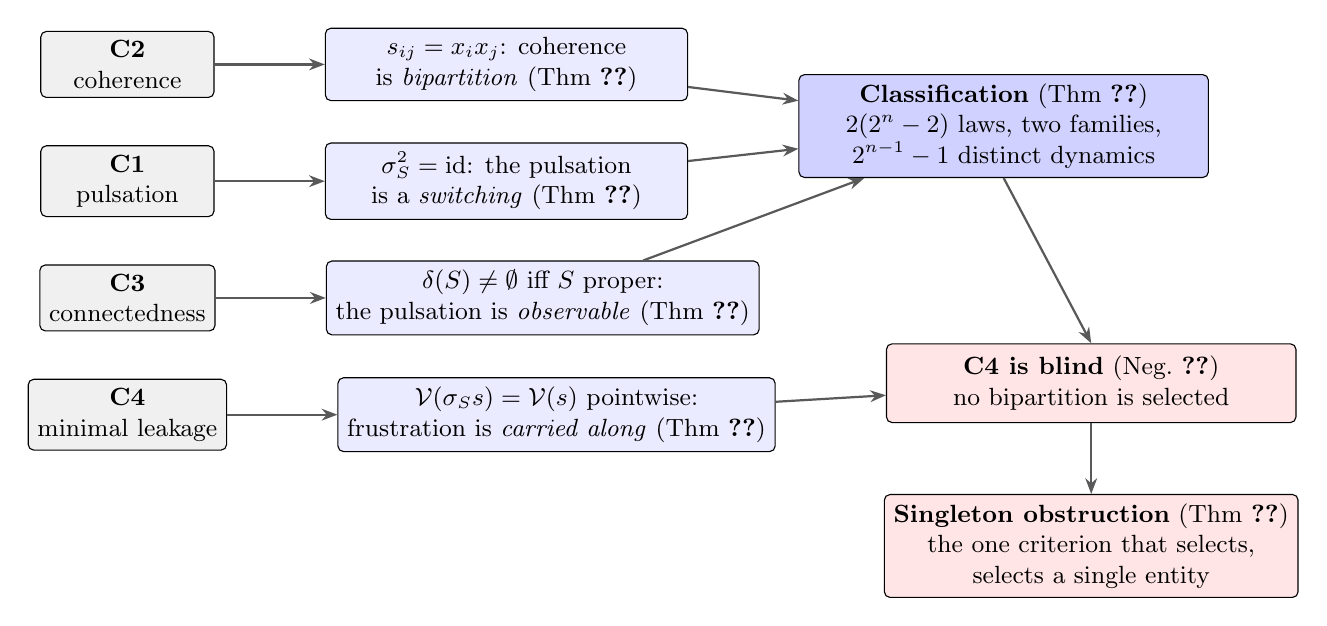
\begin{tikzpicture}[
  font=\small,
  node distance=6mm,
  ax/.style={draw, rounded corners=2pt, fill=gray!12, minimum width=22mm, minimum height=8mm, align=center},
  fact/.style={draw, rounded corners=2pt, fill=blue!8, minimum width=46mm, minimum height=9mm, align=center},
  res/.style={draw, rounded corners=2pt, fill=blue!18, minimum width=52mm, minimum height=10mm, align=center},
  neg/.style={draw, rounded corners=2pt, fill=red!10, minimum width=52mm, minimum height=10mm, align=center},
  ar/.style={-{Stealth[length=2mm]}, thick, gray!70!black}
]

\node[ax] (c2) {\textbf{C2}\\coherence};
\node[ax, below=of c2] (c1) {\textbf{C1}\\pulsation};
\node[ax, below=of c1] (c3) {\textbf{C3}\\connectedness};
\node[ax, below=of c3] (c4) {\textbf{C4}\\minimal leakage};

\node[fact, right=14mm of c2] (f2) {$s_{ij}=x_ix_j$: coherence\\ is \emph{bipartition} (Thm~\ref{thm:bipartition})};
\node[fact, right=14mm of c1] (f1) {$\sigma_S^2=\mathrm{id}$: the pulsation\\ is a \emph{switching} (Thm~\ref{thm:involution})};
\node[fact, right=14mm of c3] (f3) {$\delta(S)\neq\emptyset$ iff $S$ proper:\\ the pulsation is \emph{observable} (Thm~\ref{thm:trivial})};
\node[fact, right=14mm of c4] (f4) {$\mathcal{V}(\sigma_S s)=\mathcal{V}(s)$ pointwise:\\ frustration is \emph{carried along} (Thm~\ref{thm:invariance})};

\node[res, right=14mm of f1, yshift=7mm] (cl) {\textbf{Classification}\ (Thm~\ref{thm:classification})\\ $2(2^n-2)$ laws, two families,\\ $2^{n-1}-1$ distinct dynamics};
\node[neg, right=14mm of f4, yshift=4mm] (n1) {\textbf{C4 is blind}\ (Neg.~\ref{neg:C4blind})\\ no bipartition is selected};
\node[neg, below=9mm of n1] (n2) {\textbf{Singleton obstruction}\ (Thm~\ref{thm:singleton})\\ the one criterion that selects,\\ selects a single entity};

\draw[ar] (c2) -- (f2);
\draw[ar] (c1) -- (f1);
\draw[ar] (c3) -- (f3);
\draw[ar] (c4) -- (f4);
\draw[ar] (f2) -- (cl);
\draw[ar] (f1) -- (cl);
\draw[ar] (f3) -- (cl);
\draw[ar] (f4) -- (n1);
\draw[ar] (n1) -- (n2);
\draw[ar] (cl.south) -- (n1.north);

\end{tikzpicture}
\caption{Logical architecture of D68. Each axiom contributes exactly one structural fact. C1, C2 and C3 compose into the complete classification of pulsation laws; C4 contributes the invariance that makes the classification survive frustration and, by the same token, makes C4 itself incapable of selecting among the classified dynamics. The singleton obstruction closes the one remaining family of selection criteria.}
\label{fig:chain}
\end{figure}

\subsection{Notational discipline}
\label{subsec:notation}

Throughout this document, $\Kfour$ denotes the complete signed graph on four vertices and six edges, identified in the corpus with the electron prototype~\citep{D01,D16}. Results stated for general $\Kn$ concern the abstract complete signed graph on $n$ vertices and carry no nucleon-level interpretation. Nucleon-level hierarchical closures, written $K_{\mathrm{nuc}}$ in the corpus, are not treated in this document at all, and no statement here should be read as applying to them. The distinction matters: $\Coh(\Kfour)\cong\mathbb{Z}_2^3\rtimes V_4$ (D61~\citep{D61}) is a statement about the electron closure specifically.

\subsection{Epistemic status of every claim in this document}

The programme's stratification is applied without exception. Table~\ref{tab:status} is the complete inventory.

\begin{table}[h]
\centering
\small
\begin{tabular}{llp{6.8cm}}
\toprule
\textbf{Claim} & \textbf{Status} & \textbf{Basis} \\
\midrule
Theorem~\ref{thm:bipartition} & Unconditional theorem & Harary~\citep{Harary1953}; exhaustive to $n=6$ \\
Theorem~\ref{thm:involution} & Unconditional theorem & Two-line proof; $128/128$ checks \\
Theorem~\ref{thm:trivial} & Unconditional theorem & Exhaustive; $\{\emptyset,V\}$ exactly \\
Theorem~\ref{thm:classification} & Unconditional theorem & Exhaustive over $234\,256$ laws, $n=4$; $n\le6$ \\
Proposition~\ref{prop:orbits} & Unconditional theorem & Re-derivation of D60; checked by hand in \S\ref{sec:worked} \\
Theorem~\ref{thm:invariance} & Unconditional theorem & Two-line proof; $32\,768$ checks at $n=5$ \\
Negative Result~\ref{neg:C4blind} & Established negative result & Exhaustive, $n=4,5$ \\
Theorem~\ref{thm:singleton} & Unconditional theorem & Proved here for all $n$; verified to $n=7$ \\
Corollary~\ref{cor:composite} & Unconditional theorem & Immediate from Theorem~\ref{thm:invariance} \\
Negative Result~\ref{neg:C5dead} & Established negative result & Consequence of Theorem~\ref{thm:singleton} \\
Erratum~\ref{err:D46table}, \ref{err:D46lemma} & Corrections to D46 & Verified against the D46 source \\
Erratum~\ref{err:D43sum} & Correction to D43 & Arithmetic, verified against the D43 source \\
Remark~\ref{rem:101} & Established identity & $101 = n_K + (\Delta n+1)^2$, direct \\
Remark~\ref{rem:c3} & Clarification of D43 & Hierarchical reading; no result changed \\
OP-D68-7 & Divergence of definition & D46 vs.\ this document; not adjudicated here \\
Appendix~\ref{app:ontology} & \textbf{Motivation, not proof} & Philosophical argument; no result depends on it \\
OP-D68-1 to OP-D68-6 & Open problems & Stated, not resolved \\
\bottomrule
\end{tabular}
\caption{Complete epistemic inventory of D68. No claim in this document holds a status not listed here.}
\label{tab:status}
\end{table}

\subsection{A retraction made in the course of this work}

In the course of the investigation reported here, the author's working hypothesis was that no quantity constructible from C2 and C4 could discriminate between candidate pulsation bipartitions. That hypothesis is false, and the counterexample arose within the same investigation: the functional $\cross(S)$ of Section~\ref{sec:obstruction} is built exclusively from the frustrated triangles, and it discriminates perfectly, in $1243$ of $1243$ tested cases. What disqualifies it is not failure to discriminate but the form of what it selects. The corrected statement is Theorem~\ref{thm:singleton}, and it is a stronger result than the one originally sought. The episode is recorded because a discarded hypothesis that was wrong for an interesting reason belongs in the record.

% ============================================================
\section{Prerequisites, stated in full}
\label{sec:prereq}
% ============================================================

This section is self-contained: a reader with no prior exposure to the corpus should be able to proceed from here.

\subsection{The four axioms}

\begin{itemize}
\item[\textbf{C1}] \emph{Pulsation.} Existence is instantiated as a repeatable, non-trivial alternation between two discrete states, independent of any pre-existing temporal metric. The alternation is not a fixed point.
\item[\textbf{C2}] \emph{Coherence.} Admissible configurations are those in which every elementary closed circuit carries a positive sign product. On a complete graph this is the condition that every triangle be positive.
\item[\textbf{C3}] \emph{Connectedness.} The structure is a single connected signed graph; no component stands apart.
\item[\textbf{C4}] \emph{Minimal leakage.} Among admissible structures, those realised are the ones minimising the fraction of circuits violating C2. The residual is the logical leakage $\etaL$~\citep{D08}.
\end{itemize}

\subsection{Signed graphs, coherence, switching}

\begin{definition}[Signed complete graph]
Let $V=\{0,\dots,n-1\}$ and let $E$ be the $\binom{n}{2}$ unordered pairs. A sign configuration is a map $s:E\to\{+1,-1\}$, written $s_{ij}$.
\end{definition}

\begin{definition}[Coherence]
A triangle $T=\{i,j,k\}$ is \emph{coherent} if $s_{ij}s_{ik}s_{jk}=+1$ and \emph{violated} otherwise. The configuration $s$ is coherent, written $s\in\Coh(\Kn)$, if every triangle is coherent. This is Harary balance restricted to complete graphs~\citep{Harary1953,Zaslavsky1982}.
\end{definition}

\begin{definition}[Switching]
\label{def:switching}
For $S\subseteq V$, the \emph{switching} $\sigma_S$ acts on configurations by
\[
(\sigma_S s)_{ij} \;=\;
\begin{cases}
-s_{ij} & \text{if exactly one of } i,j \text{ lies in } S,\\
\;\;\;s_{ij} & \text{otherwise.}
\end{cases}
\]
The set of edges with exactly one endpoint in $S$ is the \emph{cut} $\delta(S)$.
\end{definition}

Two remarks on Definition~\ref{def:switching} are used constantly and should be internalised at once. First, $\sigma_S=\sigma_{V\setminus S}$ identically, since an edge has exactly one endpoint in $S$ if and only if it has exactly one endpoint in the complement. A switching is therefore an operation attached to an unordered bipartition, not to a distinguished side. Second, $\sigma_S\circ\sigma_S=\mathrm{id}$ for every $S$: switching is an involution.

\subsection{What counts as a state, and what does not}

One point of interpretation governs everything that follows and is worth stating before any theorem. In \PDL, a relation carries no state of its own. Its sign records whether its two relata are alike or unlike; it does not record which state either of them holds. The observable content of a configuration is therefore the collection of edge signs, not the assignment of vertex values. Two vertex assignments that induce the same edge signs describe the same world, however different they look. This is not a modelling convenience adopted here for the sake of the argument: it is the relational commitment of the programme, present from D01 onward, and Theorem~\ref{thm:trivial} is simply what it costs.

\subsection{Vertex-induced configurations}

\begin{definition}
A configuration is \emph{vertex-induced} if there exists $x:V\to\{+1,-1\}$ with $s_{ij}=x_ix_j$ for all edges.
\end{definition}

That every vertex-induced configuration is coherent is immediate and was already recorded in D67~\citep{D67}: the product around a triangle is $x_i^2x_j^2x_k^2=+1$. The converse is Harary's theorem and is central to what follows.

% ============================================================
\section{Coherence is bipartition}
\label{sec:bipartition}
% ============================================================

\begin{theorembox}[Theorem~\ref{thm:bipartition}]
A configuration on $\Kn$ is coherent if and only if it is vertex-induced. Consequently $|\Coh(\Kn)|=2^{\,n-1}$, and every coherent configuration has exactly two preimages, $x$ and $-x$. The relational state of a C2-admissible structure is therefore a \emph{bipartition of its entities}, not a list of edge signs.
\end{theorembox}

\begin{theorem}
\label{thm:bipartition}
As stated in the box above.
\end{theorem}

\begin{proof}
Sufficiency is the computation just given. For necessity, fix a vertex $0$ and set $x_0=+1$, $x_i=s_{0i}$ for $i\neq0$. For any edge $\{i,j\}$ with $i,j\neq0$, coherence of the triangle $\{0,i,j\}$ gives $s_{0i}s_{0j}s_{ij}=+1$, hence $s_{ij}=s_{0i}s_{0j}=x_ix_j$; and $s_{0i}=x_0x_i$ by construction. So $s$ is vertex-induced. The map $x\mapsto s$ is two-to-one, since $x$ and $-x$ give the same $s$ and no other $x'$ does (fixing $x_0$ determines the rest). Hence $|\Coh(\Kn)|=2^n/2=2^{n-1}$.
\end{proof}

This matches the count recorded in D66~\citep{D66} and is verified exhaustively for $n=3,4,5,6$ by \texttt{script1}, Part~1, together with the two-to-one preimage property. It is carried out by hand for $n=4$ in Section~\ref{subsec:worked_coh}.

\begin{remark}
The content of Theorem~\ref{thm:bipartition} is ontological as much as combinatorial. If a relation is the product of the states of its relata, C2 is not an independent constraint but a consequence of that reading. This is a possible reformulation of the axiomatic base, not an economy of axioms, and it is not adopted here: C2 is used throughout the corpus from D01 onward, and replacing it is a decision of a different order from the results of this document. It is recorded as a direction in OP-D68-6.
\end{remark}

% ============================================================
\section{The pulsation is a switching}
\label{sec:pulsation}
% ============================================================

\begin{theorembox}[Theorem~\ref{thm:involution}]
For every $S\subseteq V$, the switching $\sigma_S$ maps $\Coh(\Kn)$ into itself and satisfies $\sigma_S^2=\mathrm{id}$. Consequently every fixed subset $S$ generates an exact logical two-cycle, and C1 is satisfied by construction for any $S$.
\end{theorembox}

\begin{theorem}
\label{thm:involution}
As stated.
\end{theorem}

\begin{proof}
If $s_{ij}=x_ix_j$, define $x'_i=-x_i$ for $i\in S$ and $x'_i=x_i$ otherwise. Then $x'_ix'_j$ equals $-x_ix_j$ exactly when precisely one of $i,j$ lies in $S$, which is the definition of $\sigma_S$. So $\sigma_S s$ is vertex-induced, hence coherent by Theorem~\ref{thm:bipartition}. Applying the same construction twice restores $x$, giving $\sigma_S^2=\mathrm{id}$.
\end{proof}

Verified exhaustively at $n=4$ over all $16$ subsets and all $8$ coherent configurations: $128/128$ for coherence preservation and $128/128$ for involutivity (\texttt{script1}, Part~2).

\begin{remark}
The two-cycle demanded by C1 is thus not a delicate dynamical achievement but an automatic consequence of the switching structure. What C1 constrains is not \emph{whether} a two-cycle exists but \emph{which} subsets produce a non-trivial one. That is the subject of the next section.
\end{remark}

% ============================================================
\section{Universal simultaneous inversion is the trivial element}
\label{sec:trivial}
% ============================================================

\begin{theorembox}[Theorem~\ref{thm:trivial}]
$\sigma_S$ acts as the identity on $\Coh(\Kn)$ if and only if $S\in\{\emptyset,V\}$. Hence the simultaneous inversion of the state of every entity leaves the relational configuration strictly unchanged: it is a fixed point, and is excluded by C1 not as incoherent but as empty.
\end{theorembox}

\begin{theorem}
\label{thm:trivial}
As stated.
\end{theorem}

\begin{proof}
If $S=\emptyset$ or $S=V$, no edge has exactly one endpoint in $S$, so $\delta(S)=\emptyset$ and $\sigma_S=\mathrm{id}$. Conversely, if $S$ is proper and non-empty, pick $i\in S$ and $j\notin S$; on a complete graph the edge $\{i,j\}$ exists and lies in $\delta(S)$, so $\sigma_S$ changes at least one sign.
\end{proof}

Verified exhaustively at $n=4$: exactly two subsets act trivially, namely $\emptyset$ and $V$ (\texttt{script1}, Part~3).

\begin{remark}[The role of C3]
\label{rem:C3}
The converse direction of the proof used the existence of an edge between $S$ and its complement. On a complete graph this is automatic; on a general connected graph it is exactly connectedness. On a disconnected graph it fails: for the graph with components $\{0,1\}$ and $\{2,3\}$, the proper non-empty subsets $\{0,1\}$ and $\{2,3\}$ both have empty cut and act trivially (\texttt{script1}, Part~3, reports $0$ such subsets for the connected path $0$--$1$--$2$--$3$ and $2$ for the disconnected graph). C3 is therefore precisely what makes the pulsation observable, and it earns its place in the axiom list on this ground independently of the roles it plays elsewhere in the corpus.
\end{remark}

\begin{remark}[Relation to D46]
\label{rem:D46}
Theorem~\ref{thm:trivial} is the combinatorial form of a result the corpus already possessed. D46~\citep{D46} established that the global phase $\psi\mapsto e^{i\alpha}\psi$ is unobservable and that the physical state space is the orbit space of the $\mathrm{U}(1)$ action. What is added here is the identification of the \emph{source} of that unobservability in the sign structure itself: because a relation is the product of two states, inverting both leaves the product fixed. The global phase is not an additional feature of the amplitude formalism; it is the shadow, in the amplitude formalism, of the fact that vertex states are not relational data.
\end{remark}

\begin{remark}[Why the naive reading fails, and where it is right]
\label{rem:naive}
A reader may object that inverting both terms of a relation should reverse its sense. It does not, and the reason is worth stating plainly. A \PDL\ relation does not encode which state each relatum holds; it encodes whether they are \emph{alike or unlike}. Two magnets both reversed remain aligned; two people who both change their minds still agree. To construct a relation that would reverse under simultaneous inversion, one would have to compare each entity to something that did not invert --- a fixed background, an absolute frame, a third term standing outside the relation. That is exactly what the programme forbids from its first line. The impossibility is therefore not a modelling convenience but a direct consequence of the relational commitment. An analogy sometimes offered, that of a room in which everyone turns to face the opposite direction, is misleading and should be avoided: facing compares an orientation to a \emph{position}, which does not turn, so the analogy smuggles in the very third term the theorem excludes.
\end{remark}

% ============================================================
\section{Complete classification of C1-admissible pulsation laws}
\label{sec:classification}
% ============================================================

\subsection{The general flip law}

To classify pulsation laws without prejudging their form, we parametrise them as generally as the notion allows and then let the classification eliminate.

\begin{definition}[Flip law]
\label{def:law}
A \emph{flip law} assigns to each entity $i$ a pair $(p_i,\varphi_i)$, where $p_i\in\{1,2,3,\dots\}\cup\{\infty\}$ is a period and $\varphi_i\in\{0,\dots,p_i-1\}$ a phase offset. Entity $i$ changes state at every step $u\ge1$ with $u\equiv\varphi_i \pmod{p_i}$; if $p_i=\infty$ it never changes state. Writing $f_i(t)$ for the number of changes of $i$ in $[1,t]$, the \emph{parity set} is
\[
F_t \;=\; \{\, i \in V \;:\; f_i(t) \text{ is odd} \,\},
\]
and the relational state at step $t$ is $s_t=\sigma_{F_t}s_0$.
\end{definition}

\begin{definition}[C1-admissibility]
A flip law is \emph{C1-admissible} if the sequence $(s_t)_{t\ge0}$ has exact period $2$ and is not constant.
\end{definition}

The index $t$ in Definition~\ref{def:law} is scaffolding, not structure. It is used to enumerate laws; the laws that survive, as Theorem~\ref{thm:classification} shows, reduce to a single involutive switching and require no global clock. This is consistent with C1's stipulation that the alternation be independent of any pre-existing temporal metric, and the reader should not read a cosmic counter into the parametrisation.

\subsection{The classification}

\begin{theorembox}[Theorem~\ref{thm:classification}]
On $n$ entities the C1-admissible flip laws number exactly $2(2^n-2)$. They fall into exactly two families and no third:
\begin{enumerate}
\item[(i)] \emph{uniform period two with binary phase}: $p_i=2$ for every $i$, with $\varphi_i\in\{0,1\}$ and both phase classes non-empty;
\item[(ii)] \emph{degenerate}: $p_i=1$ for $i\in S$ and $p_i=\infty$ otherwise, with $S$ proper and non-empty.
\end{enumerate}
Each family contains $2^n-2$ laws. The two families generate \emph{identical} relational sequences, and the total number of distinct relational dynamics is $2^{n-1}-1=|\Coh(\Kn)|-1$. In family~(i), every entity changes state exactly once per relational cycle.
\end{theorembox}

\begin{theorem}
\label{thm:classification}
As stated.
\end{theorem}

\begin{proof}
Since $\sigma_{F}=\sigma_{V\setminus F}$ and $\sigma_F^2=\mathrm{id}$, the relational state depends on $F_t$ only through its class modulo complementation, and the group generated is elementary abelian. Exact period two with non-constancy therefore requires $\sigma_{F_{t+1}}\neq\sigma_{F_t}$ for some $t$ and $\sigma_{F_{t+2}}=\sigma_{F_t}$ for all $t$.

For family~(ii), $f_i(t)=t$ for $i\in S$ and $f_i(t)=0$ otherwise, so $F_t=S$ for odd $t$ and $F_t=\emptyset$ for even $t$. The sequence alternates between $s_0$ and $\sigma_S s_0$, of exact period two, non-constant precisely when $\delta(S)\neq\emptyset$, that is (Theorem~\ref{thm:trivial}) when $S\notin\{\emptyset,V\}$. This gives $2^n-2$ laws.

For family~(i), let $A=\{i:\varphi_i=0\}$ and $B=V\setminus A$. With $p_i=2$ and $\varphi_i=0$, $f_i(t)=\lfloor t/2\rfloor$, odd exactly when $t\equiv2,3\pmod4$; with $\varphi_i=1$, $f_i(t)=\lceil t/2\rceil$, odd exactly when $t\equiv1,2\pmod4$. Hence $F_0=\emptyset$, $F_1=B$, $F_2=V$, $F_3=A$, and the pattern repeats with period four in $F$ but period two in the relational state, since $\sigma_\emptyset=\sigma_V=\mathrm{id}$ and $\sigma_A=\sigma_B$. The sequence is $s_0,\ \sigma_B s_0,\ s_0,\ \sigma_B s_0,\dots$, non-constant precisely when $A\notin\{\emptyset,V\}$; this gives $2^n-2$ laws. Setting $A=S$ makes the two sequences identical, which establishes the claimed coincidence of the families. At $t=2$ each entity has changed state exactly once, and the relational state has returned.

That no third family exists, and that no other period assignment is admissible, is established by exhaustive enumeration: at $n=4$, over all $22^4=234\,256$ laws with $p\in\{\infty,1,\dots,6\}$ and all admissible offsets, exactly $28=2(2^4-2)$ are C1-admissible, of which $14$ lie in family~(i) and $14$ in family~(ii), and $0$ in neither (\texttt{script2}, Parts~2--3). The count $2(2^n-2)$ and the distinct-dynamics count $2^{n-1}-1$ are confirmed at $n=3,4,5,6$ (\texttt{script2}, Part~5), yielding $12,28,60,124$ and $3,7,15,31$ respectively.
\end{proof}

\subsection{Reading the classification}

Three consequences deserve to be stated separately.

The first is that a homogeneous rhythm is empty. If every entity shares one period, whatever that period, then $F_t\in\{\emptyset,V\}$ at all times and the relational state never moves. This holds for $p=1,\dots,6$ by direct computation (\texttt{script1}, Part~5b) and by the argument above in general. Heterogeneity is not an optional refinement; without it there is no dynamics at all.

The second is that heterogeneity of \emph{period} does not work either. Exhaustive search at $n=4$ over all assignments with finite periods in $\{1,\dots,4\}$ yields relational periods $1,3,4,8,12,24$ --- and period $2$ never occurs (\texttt{script1}, Part~5c: $0$ of $256$). Nor does randomness: $0$ of $20\,000$ random flip sequences produce an exact non-constant two-cycle (\texttt{script1}, Part~5d). What is required is heterogeneity of \emph{phase}, at a common period.

The third is that family~(ii), which appears to require a class of entities that never change, is a description rather than a fact. Its relational sequence is identical to that of family~(i), in which all entities are identical in nature and all change state (verified for all $14$ proper non-empty subsets at $n=4$; \texttt{script2}, Part~4, claim S1). The static camp is an artefact of the chosen description, and family~(i) is the canonical form precisely because it introduces no distinction without an observable difference.

\begin{remark}[No entity and no camp is privileged]
Since $\sigma_A=\sigma_{V\setminus A}$, there is no fact of the matter as to which phase class moves first, or which of the two is ``in advance''. The opposition of phase is real; its orientation is not. This is the same principle as Theorem~\ref{thm:trivial}, applied to the rhythm rather than to the states.
\end{remark}

\begin{remark}[Relation to $T^2=-I_2$]
\label{rem:T2}
In family~(i) the vertex pattern is completely inverted at $t=2$, every entity having changed state exactly once (\texttt{script2}, Part~4, claim S2), and the completely inverted state is relationally identical to the starting state. The observable content lies in the intermediate state at $t=1$. A full return therefore requires two logical steps and carries the sign structure that D33 established as $T^2=-I_2$ and D46 lifted to the Hopf fibration. The present derivation reaches the same structure from the switching side, with no amplitude formalism in play.
\end{remark}

\subsection{Recovering the orbit decomposition of D60}

\begin{proposition}
\label{prop:orbits}
The distinct pulsation dynamics on $\Kn$ are in bijection with the non-trivial cuts, hence with $\Coh(\Kn)\setminus\{s_{\mathrm{ref}}\}$. For $n=4$ they classify by cut size as $0|4\to1$, $1|3\to4$, $2|2\to3$, reproducing exactly the $S_4$-orbit decomposition $1+3+4$ of D60~\citep{D60}. The three $2|2$ cuts together with the empty cut form a Klein four-group under symmetric difference.
\end{proposition}

\begin{proof}
Theorem~\ref{thm:classification} identifies a dynamics with the switching $\sigma_S$, hence with $S$ modulo complementation, hence with a bipartition; Theorem~\ref{thm:bipartition} identifies bipartitions with coherent configurations, the trivial cut corresponding to the reference configuration. The count by size follows from $\binom{4}{0}=\binom{4}{4}=1$ giving one class, $\binom{4}{1}=\binom{4}{3}=4$ giving four, and $\binom{4}{2}=6$ giving three after quotienting by complementation. Closure of the even cuts under symmetric difference is direct. Verified in \texttt{script1}, Part~4, and checked configuration by configuration against D60's own listing in Section~\ref{subsec:worked_orbits}.
\end{proof}

\begin{remark}
Proposition~\ref{prop:orbits} changes the reading of D60 without changing any of its results. The decomposition $1+3+4$ was obtained there as a statement about the action of $S_4$ on $\Coh(\Kfour)$; it is here seen to be a classification of \emph{pulsation laws} by the size of the bipartition they realise. The structure of the electron closure and its rhythm are not two facts but one fact counted twice. Whether the Klein group of even cuts coincides, as an action on the four-element orbit, with the $V_4$ of D60 and with the three perfect matchings identified as real axes in D61~\citep{D61} is not established here; see OP-D68-2.
\end{remark}

% ============================================================
\section{The frustrated regime}
\label{sec:frustration}
% ============================================================

Everything above concerns configurations satisfying C2 exactly. The universe described by the corpus does not: C4 minimises a residual leakage $\etaL\neq0$~\citep{D08}. If the classification collapsed under frustration it would describe a toy model. It does not, and the reason is a single parity observation.

\begin{theorembox}[Theorem~\ref{thm:invariance}]
Let $s$ be any configuration on $\Kn$ and let $\mathcal{V}(s)$ be its set of violated triangles. Then $\mathcal{V}(\sigma_S s)=\mathcal{V}(s)$ for every $S\subseteq V$ --- not merely equal in cardinality, but the same triangles, one by one.
\end{theorembox}

\begin{theorem}
\label{thm:invariance}
As stated.
\end{theorem}

\begin{proof}
Let $T=\{i,j,k\}$ and let $m=|T\cap S|$. The number of edges of $T$ lying in $\delta(S)$ is $2$ if $m\in\{1,2\}$ and $0$ if $m\in\{0,3\}$; it is never $1$ or $3$, since a triangle has an even number of edges in any cut. The sign product of $T$ is therefore multiplied by $(-1)^0$ or $(-1)^2$, that is by $+1$, in all cases.
\end{proof}

Verified exhaustively for $n=3,4,5$ over every configuration and every subset, $32\,768$ checks at $n=5$, for the set and not merely the count (\texttt{script3}, Part~1).

\begin{corollary}
\label{cor:notoy}
The classification of Theorem~\ref{thm:classification} is independent of frustration.
\end{corollary}

\begin{proof}
The classification used only the cut structure and the involutivity of switching, neither of which refers to coherence. Verified directly by re-running the enumeration on frustrated reference configurations: at $n=4$ with $v=0,2,4$ violated triangles, each gives $28$ admissible laws, $14+14+0$, and $7$ distinct dynamics (\texttt{script3}, Part~2).
\end{proof}

\begin{remark}[The frustration spectrum and $s\mapsto-s$]
\label{rem:spectrum}
The number of switching classes of $\Kn$ is $2^{\binom{n-1}{2}}$, each of size $2^{n-1}$, and every class has a unique representative with all edges at vertex $0$ positive. Their frustration spectra are symmetric: $(1,6,1)$ at $n=4$ for $v=0,2,4$, and $(1,10,15,12,15,10,1)$ at $n=5$ for $v=0,3,4,5,6,7,10$ (\texttt{script3}, Part~4). The symmetry is $v\mapsto\binom{n}{3}-v$, which is exactly the global edge inversion $s\mapsto-s$: a triangle has three edges, so every triangle product is inverted. C4 breaks this symmetry by selecting the low-frustration end, and the anti-coherent regime is thereby excluded --- not by C2, which the inversion preserves as a symmetry of the class structure, but by the minimisation itself.
\end{remark}

% ============================================================
\section{Negative result: C4 does not select the bipartition}
\label{sec:blind}
% ============================================================

\begin{negbox}[Negative Result~\ref{neg:C4blind}]
The frustration count is identical across all $2^{n-1}-1$ candidate pulsation bipartitions, at every step of the pulsation. C4 therefore cannot select among them. The pulsation bipartition is undetermined by C1--C4.
\end{negbox}

\begin{negresult}
\label{neg:C4blind}
As stated.
\end{negresult}

\begin{proof}
Immediate from Theorem~\ref{thm:invariance}: the pulsation acts by switching, which leaves $\mathcal{V}(s)$ pointwise fixed. Every candidate dynamics therefore visits configurations with the same violated set, hence the same $\etaL$, at every step.
\end{proof}

Verified by an independent route: over all configurations at $n=4$ and $n=5$, the number of \emph{distinct} frustration counts across the $14$ and $30$ candidate bipartitions respectively is exactly $1$ (\texttt{script3}, Part~3).

\begin{remark}[Conservation is what prevents selection]
This deserves to be read correctly, because the natural expectation runs the other way. One might hope that a conservation law would constrain the pattern. The opposite holds. A conservation law states that a quantity does not change under the evolution; it says nothing about which value that quantity had to take. Conservation constrains becoming, not choosing. Structurally, conservation laws arise from symmetries, and a symmetry is an assertion of indifference between options. To seek, in the statement ``these options are equivalent'', a reason to prefer one of them, is to seek what the statement denies. What selects, in physics, is never a conservation but a breaking. Negative Result~\ref{neg:C4blind} is the precise form this takes in \PDL: the leakage is \emph{too} well conserved to discriminate.
\end{remark}

% ============================================================
\section{The singleton obstruction theorem}
\label{sec:obstruction}
% ============================================================

Negative Result~\ref{neg:C4blind} does not close the question, because a quantity may be built from the violated triangles that is not itself switching-invariant. Exactly one such quantity arises naturally, and this section determines what it does.

\subsection{The crossing functional}

\begin{definition}
\label{def:cross}
Let $S$ be a proper non-empty subset of $V$ and $\mathcal{V}$ a set of triangles. A triangle $T$ is \emph{crossing} for $S$ if its vertices are split by $S$, equivalently if exactly two of its edges lie in $\delta(S)$; otherwise it is \emph{internal}. Write
\[
\cross(S)=\#\{T\in\mathcal{V}: T \text{ crossing}\},\qquad
\mono(S)=|\mathcal{V}|-\cross(S).
\]
\end{definition}

The functional $\cross$ is built exclusively from the violated triangles, hence from C4, and it depends on $S$; it is not switching-invariant. It is the only candidate this investigation produced that is both admissible under the programme's anchoring requirement --- no quantity constructed for the occasion --- and capable of discriminating. Minimising $\cross(S)$ has a transparent reading: the frustration should sit away from the pulsating boundary.

\begin{corollary}[Composite criteria cannot rank differently]
\label{cor:composite}
Let $F$ be any functional of the form $F(S)=G(\cross(S),|\mathcal{V}|)$ with $G$ strictly monotone in its first argument. Then $F$ induces the same ranking of bipartitions as $\cross$ alone. In particular, no combination of the total tension with the crossing/internal split --- ratio, difference, product, or otherwise --- can select differently from $\cross$.
\end{corollary}

\begin{proof}
By Theorem~\ref{thm:invariance}, $|\mathcal{V}|$ is the same for every candidate $S$; it enters $G$ as a constant. A strictly monotone function of $\cross(S)$ alone induces the ranking of $\cross(S)$.
\end{proof}

\subsection{Two-graphs}

The violated sets arising from actual configurations are not arbitrary triangle sets, and this is what makes the obstruction theorem true.

\begin{definition}[Two-graph]
A set $\Delta$ of $3$-subsets of $V$ is a \emph{two-graph} if every $4$-subset of $V$ contains an even number of members of $\Delta$~\citep{Seidel1976,Taylor1977}.
\end{definition}

\begin{proposition}
\label{prop:twograph}
The sets $\mathcal{V}(s)$ arising from configurations on $\Kn$ are exactly the two-graphs on $V$, and there are $2^{\binom{n-1}{2}}$ of them.
\end{proposition}

\begin{proof}
For $Q=\{i,j,k,l\}$, the product of the four triangle products over the four triangles in $Q$ counts each of the six edges of $Q$ exactly twice, hence equals $+1$; so the number of violated triangles in $Q$ is even. The correspondence with switching classes, and the count, is classical~\citep{Seidel1976}.
\end{proof}

Verified exhaustively for $n=4,5,6,7$: $8$, $64$, $1024$, $32\,768$ distinct violated sets, all satisfying the parity condition (\texttt{script5}, Part~1).

\subsection{The theorem}

For a two-graph $\Delta$ and $u\in V$ write $\dtg(u)=\#\{T\in\Delta:u\in T\}$. A triangle is crossing for the singleton $\{u\}$ precisely when it contains $u$, so
\begin{equation}
\cross(\{u\})=\dtg(u).
\label{eq:singleton}
\end{equation}

\begin{theorembox}[Theorem~\ref{thm:singleton}]
Let $\Delta$ be a non-empty two-graph on $n\ge4$ vertices. Then for every $S$ with $2\le|S|\le n-2$,
\[
\min_{u\in V}\dtg(u)\;<\;\cross(S).
\]
The minimum of $\cross$ over all proper non-empty subsets is therefore attained at a cut of size one, and at no cut of any other size. The bipartition selected by minimising $\cross$ singles out one entity: the one participating least in the frustration.
\end{theorembox}

\begin{theorem}
\label{thm:singleton}
As stated.
\end{theorem}

The proof uses one preliminary lemma and then divides into the case $|S|=2$ and the case $3\le|S|\le n-3$. These two cases exhaust the range $2\le|S|\le n-2$: the first covers $|S|=2$ and, by the identity $\cross(S)=\cross(V\setminus S)$, also $|S|=n-2$; the second covers everything strictly between. For $n=4$ and $n=5$ the second case is empty and the first alone suffices, since $2\le|S|\le n-2$ then admits only $|S|\in\{2,n-2\}$.

\begin{lemma}
\label{lem:nonzero}
In a non-empty two-graph on $n\ge4$ vertices, $\dtg(u)\ge1$ for every $u$.
\end{lemma}

\begin{proof}
Suppose $\dtg(u)=0$ and let $\{p,q,r\}\subseteq V\setminus\{u\}$ be arbitrary; such a triple exists because $n\ge4$. The four triples of $Q=\{u,p,q,r\}$ are $\{p,q,r\}$ and three triples containing $u$; the latter are not in $\Delta$. Parity forces $\#(\Delta\cap Q)$ to be even, hence $\{p,q,r\}\notin\Delta$. So no triple avoiding $u$ lies in $\Delta$, and none containing $u$ does either, giving $\Delta=\emptyset$.
\end{proof}

\begin{proof}[Proof of Theorem~\ref{thm:singleton}, case $|S|=2$]
Write $S=\{u,w\}$ and partition $\Delta$ by intersection with $S$:
\[
c_0=\#\{T:T\cap S=\emptyset\},\quad
c_1^u=\#\{T:T\cap S=\{u\}\},\quad
c_1^w=\#\{T:T\cap S=\{w\}\},\quad
c_2=\#\{T:S\subseteq T\}.
\]
Since $|S|=2<3$, no triple lies inside $S$; a triple is internal exactly when it avoids $S$. Hence $\cross(S)=c_1^u+c_1^w+c_2$, while $\dtg(u)=c_1^u+c_2$ and $\dtg(w)=c_1^w+c_2$. Therefore
\[
\cross(S)-\dtg(u)=c_1^w,\qquad \cross(S)-\dtg(w)=c_1^u .
\]
If $c_1^u+c_1^w>0$, one of these is strictly positive and the claim holds. Otherwise $c_1^u=c_1^w=0$: every member of $\Delta$ contains both $u,w$ or neither. For $x,y\notin S$, parity on $\{u,w,x,y\}$ eliminates the two triples meeting $S$ in one element and gives $[\{u,w,x\}\in\Delta]=[\{u,w,y\}\in\Delta]$, so either $c_2=0$ or $c_2=n-2$. If $c_2=0$ then $\dtg(u)=0$, contradicting Lemma~\ref{lem:nonzero}. So $c_2=n-2$ and, for $n\ge5$, parity on $\{u,x,y,z\}$ with $x,y,z\notin S$ forces $c_0=0$; for $n=4$ the complement of $S$ has only two elements, so $c_0=0$ holds trivially. Then $\cross(S)=n-2\ge2$, while any $z\notin S$ has $\dtg(z)=1$. Hence $\min_u\dtg(u)\le1<n-2$ for $n\ge4$.
\end{proof}

\begin{proof}[Proof of Theorem~\ref{thm:singleton}, case $3\le|S|\le n-3$]
Write $k=|S|$, $B=V\setminus S$, so $|B|=n-k\ge3$ and, since $3\le k\le n-3$ requires $n\ge6$, we have $n-5\ge1$. Let
\[
a=\#\{T\in\Delta: T\subseteq S\},\qquad b=\#\{T\in\Delta: T\subseteq B\},
\]
so that $|\Delta|=a+b+\cross(S)$.

\emph{Forcing step.} Let $T\in\Delta$ with $T\subseteq S$ and let $y\in B$. The $4$-subset $T\cup\{y\}$ contains $T$ together with the three triples $\{p,q,y\}$ for $\{p,q\}\subset T$. Parity requires an even total; $T$ contributes one; hence an odd, and so at least one, of the three triples $\{p,q,y\}$ lies in $\Delta$. Each such triple has two vertices in $S$ and one in $B$, hence is crossing. Counting the $a(n-k)$ pairs $(T,y)$, and noting that a given crossing triple $\{p,q,y\}$ of this type arises from at most $k-2$ sets $T=\{p,q,r\}\subseteq S$, we obtain
\[
\#\{\text{crossing triples of type } (2,1)\}\;\ge\;\frac{a(n-k)}{k-2}.
\]
The symmetric argument, with $T\subseteq B$ and $x\in S$, gives
\[
\#\{\text{crossing triples of type } (1,2)\}\;\ge\;\frac{bk}{n-k-2}.
\]
Both denominators are at least $1$ because $3\le k\le n-3$. The two types are disjoint, so
\begin{equation}
\cross(S)\;\ge\;\frac{a(n-k)}{k-2}+\frac{bk}{n-k-2}.
\label{eq:forcing}
\end{equation}

\emph{Averaging step.} Each member of $\Delta$ contributes to three vertex degrees, so $\sum_{u}\dtg(u)=3|\Delta|$ and $\min_u\dtg(u)\le3|\Delta|/n$. It therefore suffices to prove $3|\Delta|/n<\cross(S)$, which after substituting $|\Delta|=a+b+\cross(S)$ is equivalent to
\begin{equation}
3(a+b)\;<\;(n-3)\,\cross(S).
\label{eq:target}
\end{equation}
If $a=b=0$ then $\cross(S)=|\Delta|>0$ and \eqref{eq:target} is immediate. Otherwise, apply \eqref{eq:forcing}. Since $k\le n-3$ gives $n-k\ge3$ and $k-2\le n-5$, the coefficient of $a$ satisfies
\[
\frac{(n-3)(n-k)}{k-2}\;\ge\;\frac{3(n-3)}{n-5}\;>\;3,
\]
the last inequality because $n-3>n-5>0$. Since $k\ge3$ gives $n-k-2\le n-5$, the coefficient of $b$ satisfies the same bound. With $a+b>0$ at least one of the two terms is strictly greater than three times its multiplicand and neither is smaller, so the inequality \eqref{eq:target} is strict, which completes the proof.
\end{proof}

Statement and proof are confirmed exhaustively: over all $32\,767$ non-empty two-graphs at $n=7$, and all non-empty two-graphs at $n=4,5,6$, the minimum of $\cross$ is attained at a singleton and at no other cut size, with no exception (\texttt{script5}, Part~2). The selected cut sizes are $\{1\}$ for all $1093$ frustrated switching classes at $n=4,5,6$ and for $150$ sampled classes at $n=7$ (\texttt{script4}, Part~4). A fully worked instance is given in Section~\ref{subsec:worked_cross}.

\subsection{Parity is the mechanism}

The theorem is false for arbitrary triangle sets. On $n=6$ with $\mathcal{V}=\{\{0,1,2\},\{3,4,5\}\}$, the $3|3$ cut $S=\{0,1,2\}$ leaves both triangles internal and gives $\cross(S)=0$, while every singleton gives $1$. That set is not a two-graph: the $4$-subset $\{0,1,2,3\}$ contains exactly one of its members, namely $\{0,1,2\}$, an odd number. The configuration is therefore not realisable on a signed graph at all.

The attribution of the effect to parity rather than to cut size is confirmed by a size-matched comparison, which is the appropriate control: uniformly random triangle sets would not have the size distribution of two-graphs, so a naive comparison could credit parity with what is merely a size effect. At $n=6$ and $n=7$, random triangle sets of exactly the sizes two-graphs attain violate the conclusion at rates up to $6.2\%$ and $9.7\%$ respectively, while no two-graph of the same size does (\texttt{script5}, Part~3). At $n=5$ the contrast is $0\%$ against $0\%$, because violations there occur only at sizes $1$ and $2$, which are not sizes of two-graphs; the attribution therefore rests on $n=6$ and $n=7$ and not on $n=5$. Exhaustive enumeration of all $2^{20}-1$ non-empty triangle sets at $n=6$ finds $1485$ violating sets, of which $0$ are two-graphs (\texttt{script5}, Part~4).

\begin{remark}[The extremal family, and a check on the proof]
\label{rem:extremal}
The minimal non-empty two-graphs are those of a single negative edge $\{u,w\}$: $\Delta=\{\{u,w,z\}:z\notin\{u,w\}\}$, of size $n-2$. Here $\min_u\dtg(u)=1$ while the best cut of size at least three achieves $\cross=3$, a gap of $2$; and there are $\binom{n}{2}$ such classes, giving $21$ at $n=7$. This is exactly the entry ``gap $2\to21$'' reported by \texttt{script5}, Part~5. The proof therefore reproduces the extremal case numerically. Across all two-graphs the gap is never $0$ and never $1$, so the inequality has margin everywhere it is applied.
\end{remark}

\subsection{Why this closes the family}

\begin{negbox}[Negative Result~\ref{neg:C5dead}]
The crossing functional selects a unique bipartition, but the bipartition it selects always isolates a single entity. In a theory whose entire content is relational, and in which no entity carries a label, designating one entity is designating an absolute frame. The construction is therefore inadmissible, and with it the whole family of criteria built from the crossing/internal split of the frustration.
\end{negbox}

\begin{negresult}
\label{neg:C5dead}
As stated.
\end{negresult}

\begin{proof}
Theorem~\ref{thm:singleton} together with \eqref{eq:singleton} identifies the selected entity as one of minimal two-graph degree. Corollary~\ref{cor:composite} extends the conclusion to every functional of the crossing count and the total tension.
\end{proof}

\begin{remark}[The escape that is not available]
One could restore competition between cut sizes by normalising $\cross(S)$ by the number of crossing triples available at that size, namely $\binom{n}{3}-\binom{k}{3}-\binom{n-k}{3}$. This is a quantity constructed for the occasion and grounded in no established corpus constraint; the programme's discipline excludes it. The balanced variant $|\cross-\mono|\to\min$ belongs to the same family, is not independently motivated, and performs strictly worse in the tests reported (\texttt{script4}, Part~1: $82.4\%$ against $100\%$ at $n=6$). It is set aside without further testing, in accordance with the rule against proposing variants of a failed family absent a structurally new ingredient.
\end{remark}

\begin{remark}[A methodological note on the falsification design]
\label{rem:method}
The design of the falsification test reported in \texttt{script4} was inadequate, and this is recorded because the inadequacy is instructive. The criterion adopted in advance was that the candidate should be judged dead if it performed no better than a null control using no frustration information. On that criterion the candidate passed comfortably: $68\%$ against $0.7\%$ at $n=7$. What killed it was a subsidiary structural test --- the cut-size profile of the selected bipartitions --- and not the pre-registered one. Further, the orbit-counting measure used there degenerates at both extremes: with a large automorphism group a single orbit is nearly automatic, and with $|\Aut|\le2$ orbits have at most two elements, so ``one orbit'' merely reports a small argmin. At $n=7$ restricted to $|\Aut|\le2$, the minimising and maximising principles both score $19/19$ and are indistinguishable. A pre-registered criterion is not a guarantee that the right thing is being measured.
\end{remark}

% ============================================================
\section{A complete worked example on \texorpdfstring{$\Kfour$}{K4}}
\label{sec:worked}
% ============================================================

This section carries every construction of the paper through explicitly on four entities. Nothing here requires a computer, and a reader who checks this section has checked the substance of Theorems~\ref{thm:bipartition}, \ref{thm:involution}, \ref{thm:trivial}, \ref{thm:classification}, \ref{thm:invariance} and~\ref{thm:singleton} in the smallest case where each has content.

\subsection{Conventions}

Take $V=\{0,1,2,3\}$ and order the six edges as
\[
e_0=\{0,1\},\quad e_1=\{0,2\},\quad e_2=\{0,3\},\quad e_3=\{1,2\},\quad e_4=\{1,3\},\quad e_5=\{2,3\},
\]
writing a configuration as the string $(s_{01},s_{02},s_{03},s_{12},s_{13},s_{23})$ with $+$ and $-$ for $+1$ and $-1$. The four triangles are $\{0,1,2\}$, $\{0,1,3\}$, $\{0,2,3\}$, $\{1,2,3\}$.

\subsection{The eight coherent configurations are the eight bipartitions}
\label{subsec:worked_coh}

By Theorem~\ref{thm:bipartition} every coherent configuration is $s_{ij}=x_ix_j$, and $x$ is determined up to global sign, so we may fix $x_0=+1$. Each of the eight remaining choices of $(x_1,x_2,x_3)$ corresponds to the subset $S=\{i:x_i=-1\}$, and $\sigma_S$ applied to the all-positive configuration gives the same result. Table~\ref{tab:worked_coh} lists all eight.

\begin{table}[h]
\centering
\small
\begin{tabular}{clllc}
\toprule
$|S|$ & $S$ & $x=(x_0,x_1,x_2,x_3)$ & $s=(s_{01},s_{02},s_{03},s_{12},s_{13},s_{23})$ & D60 orbit \\
\midrule
$0$ & $\emptyset$   & $(+,+,+,+)$ & $(+,+,+,+,+,+)$ & $\mathcal{O}_1$ \\
\midrule
$1$ & $\{0\}$       & $(-,+,+,+)$ & $(-,-,-,+,+,+)$ & $\mathcal{O}_4$ \\
$1$ & $\{1\}$       & $(+,-,+,+)$ & $(-,+,+,-,-,+)$ & $\mathcal{O}_4$ \\
$1$ & $\{2\}$       & $(+,+,-,+)$ & $(+,-,+,-,+,-)$ & $\mathcal{O}_4$ \\
$1$ & $\{3\}$       & $(+,+,+,-)$ & $(+,+,-,+,-,-)$ & $\mathcal{O}_4$ \\
\midrule
$2$ & $\{1,2\}$     & $(+,-,-,+)$ & $(-,-,+,+,-,-)$ & $\mathcal{O}_3$ \\
$2$ & $\{1,3\}$     & $(+,-,+,-)$ & $(-,+,-,-,+,-)$ & $\mathcal{O}_3$ \\
$2$ & $\{2,3\}$     & $(+,+,-,-)$ & $(+,-,-,-,-,+)$ & $\mathcal{O}_3$ \\
\bottomrule
\end{tabular}
\caption{The eight coherent configurations of $\Kfour$, each realised as a bipartition. Subsets of size $3$ are omitted because $\sigma_S=\sigma_{V\setminus S}$: for instance $\{0,1\}$ gives the same configuration as $\{2,3\}$. The last column records the $S_4$-orbit to which D60 assigns the configuration.}
\label{tab:worked_coh}
\end{table}

Each row may be checked directly. For $S=\{2,3\}$, the edges crossing the cut are $\{0,2\},\{0,3\},\{1,2\},\{1,3\}$, giving $(+,-,-,-,-,+)$; its four triangle products are $(+)(-)(-)=+$ for $\{0,1,2\}$, $(+)(-)(-)=+$ for $\{0,1,3\}$, $(-)(-)(+)=+$ for $\{0,2,3\}$ and $(-)(-)(+)=+$ for $\{1,2,3\}$. All coherent, as Theorem~\ref{thm:involution} requires.

\subsection{The orbit decomposition of D60, checked configuration by configuration}
\label{subsec:worked_orbits}

D60 lists $\Coh(\Kfour)$ as $\mathcal{O}_1=\{(+,+,+,+,+,+)\}$, together with
\[
\mathcal{O}_3=\{(-,-,+,+,-,-),\ (-,+,-,-,+,-),\ (+,-,-,-,-,+)\}
\]
and
\[
\mathcal{O}_4=\{(-,-,-,+,+,+),\ (-,+,+,-,-,+),\ (+,-,+,-,+,-),\ (+,+,-,+,-,-)\}.
\]
Comparison with Table~\ref{tab:worked_coh} shows that $\mathcal{O}_3$ is exactly the set of $2|2$ cuts and $\mathcal{O}_4$ exactly the set of $1|3$ cuts, member for member. This is Proposition~\ref{prop:orbits} in the smallest case, verified without appeal to any script.

The three even cuts $\{1,2\},\{1,3\},\{2,3\}$ together with $\emptyset$ close under symmetric difference --- for instance $\{1,2\}\,\triangle\,\{1,3\}=\{2,3\}$ --- and each is its own inverse, so they form a Klein four-group. Whether this group is \emph{the} $V_4$ of D60, as an action on $\mathcal{O}_4$, is OP-D68-2 and is not settled by this observation.

\subsection{Erratum~\ref{err:D46table} exhibited}

The all-negative configuration $(-,-,-,-,-,-)$ does not appear in Table~\ref{tab:worked_coh}, and cannot: its triangle products are $(-)(-)(-)=-1$, four times over. D46 lists it as the partner $s^{(2)}=-s^{(1)}$ of the all-positive configuration. The eight coherent configurations are not four pairs $\{s,-s\}$; they are one, four and three, as above.

The second half of Erratum~\ref{err:D46table} is also visible in Table~\ref{tab:worked_coh}. The four configurations D46 does list as coherent are the rows $S=\emptyset$, $S=\{3\}$, $S=\{2\}$ and $S=\{2,3\}$; the last is the configuration $(+,-,-,-,-,+)$, which D46 obtains as the cut $\{0,1\}$ --- the same bipartition, since $\sigma_S=\sigma_{V\setminus S}$. These four are closed under symmetric difference and form a Klein four-group. The remaining four rows of the table, $S=\{0\},\{1\},\{1,2\},\{1,3\}$, are coherent and absent from D46.

\subsection{One pulsation, followed step by step}
\label{subsec:worked_pulse}

Take the law of family~(i) with $p_i=2$ for all $i$, phase class $A=\{0,1\}$ carrying $\varphi=0$ and $B=\{2,3\}$ carrying $\varphi=1$, and start from $s_0=(+,+,+,+,+,+)$. Entities in $A$ change state at $t=2,4,\dots$; entities in $B$ at $t=1,3,\dots$. Table~\ref{tab:worked_pulse} follows four steps.

\begin{table}[h]
\centering
\small
\begin{tabular}{ccccl}
\toprule
$t$ & flips so far, $A$ & flips so far, $B$ & $F_t$ & relational state $s_t=\sigma_{F_t}s_0$ \\
\midrule
$0$ & $0$ & $0$ & $\emptyset$ & $(+,+,+,+,+,+)$ \\
$1$ & $0$ & $1$ & $\{2,3\}$   & $(+,-,-,-,-,+)$ \\
$2$ & $1$ & $1$ & $\{0,1,2,3\}$ & $(+,+,+,+,+,+)$ \\
$3$ & $1$ & $2$ & $\{0,1\}$   & $(+,-,-,-,-,+)$ \\
$4$ & $2$ & $2$ & $\emptyset$ & $(+,+,+,+,+,+)$ \\
\bottomrule
\end{tabular}
\caption{One C1-admissible pulsation on $\Kfour$. The relational state has exact period $2$ and is not constant. At $t=2$ every entity has changed state exactly once and the vertex pattern is completely inverted, yet the relational state has returned: this is Remark~\ref{rem:T2}. At $t=3$ the parity set is $\{0,1\}$, the complement of the set at $t=1$, and the two give the same configuration because $\sigma_S=\sigma_{V\setminus S}$.}
\label{tab:worked_pulse}
\end{table}

Two features of Table~\ref{tab:worked_pulse} carry the content of Section~\ref{sec:classification}. At $t=2$ the parity set is all of $V$ and the state is unchanged: this is Theorem~\ref{thm:trivial}, exhibited. And the states at $t=1$ and $t=3$ coincide although the parity sets differ, which is why the relational period is $2$ rather than $4$.

\subsection{The crossing functional, evaluated on every cut}
\label{subsec:worked_cross}

Now a frustrated example. Take $s=(-,+,+,+,+,+)$, that is, a single negative edge $\{0,1\}$. Its triangle products are $(-)(+)(+)=-$ for $\{0,1,2\}$, $(-)(+)(+)=-$ for $\{0,1,3\}$, $(+)(+)(+)=+$ for $\{0,2,3\}$ and $(+)(+)(+)=+$ for $\{1,2,3\}$. So
\[
\Delta=\mathcal{V}(s)=\bigl\{\{0,1,2\},\ \{0,1,3\}\bigr\},\qquad |\Delta|=2 .
\]
This is a two-graph: the single $4$-subset $\{0,1,2,3\}$ contains two of its members, an even number. It is the extremal family of Remark~\ref{rem:extremal} at $n=4$.

The degrees are $\dtg(0)=\dtg(1)=2$ and $\dtg(2)=\dtg(3)=1$. Table~\ref{tab:worked_cross} evaluates $\cross$ on all seven candidate bipartitions.

\begin{table}[h]
\centering
\small
\begin{tabular}{clcccc}
\toprule
$|S|$ & $S$ & $\{0,1,2\}$ crossing? & $\{0,1,3\}$ crossing? & $\cross(S)$ & $\mono(S)$ \\
\midrule
$1$ & $\{0\}$   & yes & yes & $2$ & $0$ \\
$1$ & $\{1\}$   & yes & yes & $2$ & $0$ \\
$1$ & $\{2\}$   & yes & no  & $\mathbf{1}$ & $1$ \\
$1$ & $\{3\}$   & no  & yes & $\mathbf{1}$ & $1$ \\
\midrule
$2$ & $\{0,1\}$ & yes & yes & $2$ & $0$ \\
$2$ & $\{0,2\}$ & yes & yes & $2$ & $0$ \\
$2$ & $\{0,3\}$ & yes & yes & $2$ & $0$ \\
\bottomrule
\end{tabular}
\caption{The crossing functional on all seven candidate bipartitions of $\Kfour$, for the single-negative-edge two-graph $\Delta=\{\{0,1,2\},\{0,1,3\}\}$. The minimum is $1$, attained at $\{2\}$ and $\{3\}$ and nowhere else. Both are cuts of size one, as Theorem~\ref{thm:singleton} requires.}
\label{tab:worked_cross}
\end{table}

Every row is a direct check. A triangle is crossing for $S$ when its three vertices are not all on the same side. For $S=\{2\}$, the triangle $\{0,1,2\}$ has $2$ inside and $0,1$ outside, hence crossing, while $\{0,1,3\}$ lies entirely outside $S$, hence internal; so $\cross(\{2\})=1$. For every $2|2$ cut, both violated triangles are split, since a triangle cannot fit inside a two-element set nor inside its two-element complement; so $\cross=2$ throughout.

Three points follow, and they are the whole argument of Section~\ref{sec:obstruction} in miniature. The minimum is attained only at cuts of size one, confirming Theorem~\ref{thm:singleton} at $n=4$. The selected entities, $2$ and $3$, are precisely those \emph{not} lying on the negative edge --- the entities participating least in the frustration, as \eqref{eq:singleton} predicts. And the selection designates single entities, which is what makes it inadmissible: nothing in the relational structure entitles the theory to point at entity $2$ rather than entity $3$, and indeed the signed automorphism group of this class, of order $4$, exchanges them. The criterion does not fail to discriminate; it discriminates in a way the theory is not allowed to use.

Finally, $\cross(S)$ takes the values $\{1,2\}$ across the seven bipartitions, whereas $|\Delta|=2$ is the same for all seven. This exhibits Corollary~\ref{cor:composite}: any criterion combining the total tension with the crossing count ranks the seven exactly as the middle column ranks them, because the total tension contributes a constant.

% ============================================================
\section{Corrections to earlier documents}
\label{sec:corrections}
% ============================================================

The corpus is intended to be read in order. Two errata in D46~\citep{D46} are recorded here, with the corrected statements, both verified directly against the source. A third item is not an erratum but a divergence of definition between D46 and the present document; it is recorded as Open Problem OP-D68-7 rather than as a correction, because the present document is not in a position to say which of the two definitions is the right one.

\begin{errbox}[Erratum~\ref{err:D46table}]
D46, Table~1, is incorrect in two independent ways.

\emph{First}, four of its eight rows are not coherent. The table lists the eight entries as four pulsation pairs $\{s^{(1)},s^{(2)}\}$ with $s^{(2)}=-s^{(1)}$. Direct evaluation of the four triangle products shows that each of $s^{(2)}_A,s^{(2)}_B,s^{(2)}_C,s^{(2)}_D$ violates every triangle: a triangle has three edges, so a global sign flip multiplies its product by $(-1)^3=-1$. In particular $s^{(2)}_A$ is the all-negative configuration, which is anticoherent, not coherent.

\emph{Second}, and not previously noted, the table lists only \emph{four} of the eight coherent configurations of $\Kfour$. The four it does list, $s^{(1)}_A,s^{(1)}_B,s^{(1)}_C,s^{(1)}_D$, are the switchings $\sigma_S$ of the all-positive configuration for $S=\emptyset,\{3\},\{2\},\{2,3\}$ respectively, in the representatives used in Table~\ref{tab:worked_coh} (the last is written $\{0,1\}$ if the complementary representative is preferred; $\sigma_{\{0,1\}}=\sigma_{\{2,3\}}$). These four are closed under symmetric difference and form a Klein four-group, hence a proper subgroup rather than the whole of $\Coh(\Kfour)$. The four missing coherent configurations are those obtained from $S=\{0\},\{1\},\{1,2\},\{1,3\}$.

The correct list of all eight is Table~\ref{tab:worked_coh}, and the correct decomposition is $1+3+4$ under $S_4$ (D60~\citep{D60}, re-derived here as Proposition~\ref{prop:orbits}).
\end{errbox}

\begin{erratum}
\label{err:D46table}
As stated in the box.
\end{erratum}

\begin{errbox}[Erratum~\ref{err:D46lemma}]
D46 states a lemma under the heading \emph{Global sign flip preserves triangular coherence}, asserting that if $s$ is coherent then so is $-s$. The assertion is false, and the proof printed immediately beneath it establishes the opposite, concluding that the flipped product equals $-1$ and hence that $-s$ is not coherent.

The error is confined to the heading and statement. It should be read as \emph{Global sign flip reverses triangular coherence}: the map $s\mapsto-s$ sends $\Coh(\Kfour)$ bijectively onto its complement, the set of configurations in which every triangle is violated; the two sets are disjoint and each has eight elements. On general $\Kn$ the map sends the frustration count $v$ to $\binom{n}{3}-v$ (Remark~\ref{rem:spectrum}).

It should be recorded in fairness that D46 was not unaware of the difficulty. A remark headed \emph{Resolution of the apparent contradiction} follows the lemma immediately, identifies the sign problem explicitly, and proposes to read $s$ and $-s$ as belonging to two dual coherence classes, with the physically relevant quantity being the ratio $P_2/P_1=-1$ rather than the individual products. What is corrected here is therefore the formal statement, not the mathematical awareness of the author.
\end{errbox}

\begin{erratum}
\label{err:D46lemma}
As stated in the box.
\end{erratum}

\subsection{Scope of the errata, and one divergence that is not an erratum}
\label{subsec:scope}

An earlier draft of this document asserted that neither erratum propagates, on the ground that D46's Propositions~1--3 use the equivalence $s\sim-s$ on the amplitude space $S^3$, where it is generated by $T^2=-I_2$ and is unproblematic. That assertion is withdrawn. It is correct as far as the amplitude formalism goes, but it overlooks a difference of definition at the level of edge signs, and that difference is not innocuous.

D46 defines the pulsation as the map $\Phi:s\mapsto-s$, which reverses \emph{every} edge sign, and derives from it
\[
P_1=s^{(1)}_{ij},\qquad P_2=s^{(2)}_{ij}=-s^{(1)}_{ij},\qquad\text{hence}\qquad P_2/P_1=-1 \ \text{ uniformly}.
\]
The present document derives, from C1 together with C2, that the admissible pulsation is a switching $\sigma_S$ (Theorems~\ref{thm:involution} and~\ref{thm:classification}), which reverses only the edges of the cut $\delta(S)$. These are different maps: $\Phi$ is not a switching for any $S$, which is precisely why it fails to preserve C2, whereas every $\sigma_S$ preserves it. Under a switching pulsation the ratio $P_2/P_1$ equals $-1$ on edges crossing the cut and $+1$ on edges internal to either side --- not $-1$ uniformly.

The ratio $P_2/P_1=-1$ is an input to the $(A)\wedge(B)$ stability criterion of D29, and thence to the surface microstate count of D50 and to D64. The divergence therefore reaches further than the combinatorial table, and it cannot be settled by the results of this document, which establish what C1--C4 admit as a pulsation but do not by themselves establish that the object appearing in D29's criterion is that same pulsation rather than a distinct algebraic operation on the amplitude space. It is recorded as OP-D68-7.

\subsection{A third erratum, in D43, and the resolution of a long-standing discrepancy}
\label{subsec:D43}

The correction recorded here does not concern the pulsation and would not normally belong in this document. It is included because it was found in the course of checking the numbers used above, because it removes an arithmetic obstruction from the causal chain C1--C4 $\Rightarrow G$, and because the same act of checking resolves a discrepancy that the corpus has carried across several sessions without explanation.

\begin{errbox}[Erratum~\ref{err:D43sum}]
D43~\citep{D43}, in the passage bridging the Session~21 simulation to the analytic result, states that the raw quad-mesh boundary count $E_{\mathrm{bord}}^{\mathrm{raw}}=204$ becomes the corrected count $E_{\mathrm{bord}}=329$ ``after adding the $n_K\times c=76\times3=228$ interface edges from the blocks''. The arithmetic does not close: $204+228=432$, not $329$.

The sentence is a narrative bridge, not the derivation, and the theorem it precedes is unaffected. D43's Theorem on $E_{\mathrm{bord}}$ gives
\[
E_{\mathrm{bord}} \;=\; \underbrace{n_K(1+c)}_{76\times4\;=\;304} \;+\; \underbrace{(\Delta n+1)^2}_{25} \;=\; 329,
\]
which closes exactly. The interface term is $n_K(1+c)=304$, not $n_K c=228$: each block contributes $c=3$ edges to the sea \emph{and} one further structural edge, as D43 itself states when it decomposes the three terms. The raw count $204$ plays no part in the analytic derivation; it is the boundary count of the simulated mesh, and the two quantities are not summands of one another.

The corrected sentence should read: the raw count $204$ from the simulation and the analytic count $329$ are independent determinations of different objects --- the first the topological boundary of the sea sector, the second the full boundary edge count including the block interfaces.
\end{errbox}

\begin{erratum}
\label{err:D43sum}
As stated in the box.
\end{erratum}

The distinction matters beyond the erratum. The quantity $E_{\mathrm{bord}}^{\mathrm{raw}}=204$ is what the quad-mesh formula $E_{\mathrm{bord}}=2E-4F$ returns, namely the number of edges lying on the boundary of the sea sector: with the simulation's $E_{\mathrm{sea}}=10188$ and $F_{\mathrm{sea}}=5043$, one has $2(10188)-4(5043)=204$. On a quadrangulated surface whose boundary consists of the hole circles, this is the sum of the hole perimeters. It is therefore the topological object, and it is the one to which parity arguments about the holes apply --- not $329$, which includes interface edges that are not boundary edges of the mesh.

\begin{remark}[The discrepancy of 101, resolved]
\label{rem:101}
The corpus has recorded, without explanation, that the simulation's edge count $E_{\mathrm{sea}}=10188$ exceeds the quintuplet value $R_{\mathrm{sea}}=10087$ by $101$, while D43 states that the simulation reproduces the exact counts at zero residual. Separately, the analytic boundary count exceeds the naive interface count by the same amount: $329-228=101$. The two occurrences are one and the same, and the number decomposes:
\[
101 \;=\; n_K + (\Delta n+1)^2 \;=\; 76 + 25 .
\]
The excess is exactly one structural edge per block, plus the isospin term. The simulation counts, in its edge total, the $76$ additional structural edges and the $25$ isospin edges that the quintuplet's $R_{\mathrm{sea}}$ does not carry. What was recorded as an anomaly is a decomposition. This does not by itself prove that the simulation and the quintuplet are counting the same underlying object in two conventions --- that requires checking against the Session~21 construction --- but it removes the appearance of an unexplained residual and identifies exactly what would have to be checked.
\end{remark}

\begin{remark}[On the justification of $c=3$, and the hierarchical reading]
\label{rem:c3}
D43 justifies $c=3$ by the $3$-regularity of $K_4$: each block has one outward vertex joined to the sea by three edges, the remaining three edges closing the inner triangle, so that $6=3+3$. Read as a statement about the interior of a valence core this would be untenable, since $K_{24}$ and $K_{28}$ are complete graphs on $24$ and $28$ entities and are $23$- and $27$-regular respectively, with no $K_4$ decomposition of their edge sets --- indeed $K_{24}$ admits none, since $24\not\equiv1,4\pmod{12}$.

The reading that makes the justification correct is hierarchical, and it is the one D43's own counting requires: $n_K=2n_u+n_d=76$ counts \emph{blocks}, and each entity of a valence core \emph{is} a $K_4$ closure at the level below rather than containing $K_4$ sub-blocks. There are then no $K_4$ blocks inside $K_{24}$ in the sense of an edge decomposition, while every vertex of $K_{24}$ is itself a $K_4$; the two statements are compatible and both are needed. Under this reading $c=3$ follows from the topology of the lower-level closure, exactly as D43 asserts, and the constant is legitimate.

This is a clarification of D43's wording rather than a correction of its result. It is recorded because the wording admits a reading under which the constant $c=3$ --- and hence $A=55$, $B=194$, $E_{\mathrm{bord}}=329$, $\varepsilon_{\mathrm{geom}}$ and the chain to $G$ --- would rest on a structure that is not present.
\end{remark}

Two clarifications complete the record. D60 describes the discrepancy with D46 as a potential ambiguity in the formulation of D46; it is an error rather than an ambiguity, and is corrected above. D60's own results are unaffected: the negative result there recorded --- that $s\mapsto-s$ breaks C2, verified $8/8$ --- is correct as stated, and is the same fact as Erratum~\ref{err:D46lemma}. Finally, the pulsation pairing described in D60 as the partition structure of the four-element orbit under $V_4$ is here re-derived as a statement about cut sizes; the two descriptions agree, as Section~\ref{subsec:worked_orbits} verifies member for member, and Proposition~\ref{prop:orbits} adds a reading rather than a correction.

% ============================================================
\section{Open problems}
\label{sec:open}
% ============================================================

\begin{openprobbox}[Open Problem OP-D68-1]
At $n=6$ the number of two-graphs attaining the minimal gap of $2$ between the best singleton and the best cut of size at least three is $30$, whereas the single-negative-edge family accounts for $\binom{6}{2}=15$. A second extremal family exists at $n=6$ and has not been identified. At $n=7$ the corresponding count is $21=\binom{7}{2}$, matching the single-edge family exactly, so the phenomenon is specific to $n=6$ or to small $n$. This does not affect Theorem~\ref{thm:singleton}, whose proof does not rely on the identification of the extremal families. \textbf{Priority:} low. \textbf{Entry point:} \texttt{script5}, Part~5.
\end{openprobbox}

\begin{openprobbox}[Open Problem OP-D68-2]
Determine whether the Klein four-group formed by the three even cuts of $\Kfour$ under symmetric difference (Section~\ref{subsec:worked_orbits}) coincides, as an action on the four-element orbit $\mathcal{O}_4$, with the $V_4$ of D60 and with the three perfect matchings identified as the real axes in D59 and D61. Closure under symmetric difference is verified; coincidence of the actions is not. \textbf{Priority:} medium. \textbf{Entry point:} D60, D61.
\end{openprobbox}

\begin{openprobbox}[Open Problem OP-D68-3]
Negative Result~\ref{neg:C4blind} establishes that C1--C4 do not determine the pulsation bipartition. Two readings are consistent with the present results and are not distinguished here. Either a further axiom is required, in which case Theorem~\ref{thm:invariance} localises it precisely: it must bear on the \emph{phase} assignment, which the four axioms do not see, and it cannot be any quantity invariant under switching. Or the bipartition is an irreducible contingency, and the programme has isolated the single point at which the universe was not compelled. A programme deriving structure without free parameters that terminates in one unforced binary choice has not thereby failed. The two readings differ in what would count as progress, and the distinction should be settled before further search. \textbf{Priority:} high. \textbf{Entry point:} this document, Sections~\ref{sec:blind}--\ref{sec:obstruction}.
\end{openprobbox}

\begin{openprobbox}[Open Problem OP-D68-4]
All results here concern complete signed graphs $\Kn$ and periods bounded by the enumerated range. Harary's theorem does not require completeness, so Theorem~\ref{thm:bipartition} is expected to extend to arbitrary connected signed graphs, with $|\Coh|$ replaced by the number of switching classes; this is not verified. Similarly, the exhaustive classification of Theorem~\ref{thm:classification} covers $p\le6$ at $n=4$ and $p\le3$ at $n\le6$; no proof is offered for arbitrary period. \textbf{Priority:} medium. \textbf{Entry point:} \texttt{script2}.
\end{openprobbox}

\begin{openprobbox}[Open Problem OP-D68-5]
Every quantity examined in this document is instantaneous: it is evaluated on a configuration, and the structure closes after two logical steps, retaining no trace of how many cycles have elapsed. A criterion of stability over many cycles therefore has no purchase at present, not because it is false but because nothing accumulates. Whether an object that accumulates across cycles --- a history rather than a state --- can be constructed within C1--C4 is open, and is structurally distinct from the three failed directions of Section~\ref{sec:obstruction}. \textbf{Priority:} medium. \textbf{Entry point:} Theorem~\ref{thm:classification}.
\end{openprobbox}

\begin{openprobbox}[Open Problem OP-D68-6]
Theorem~\ref{thm:bipartition} shows that if the sign of a relation is taken to be the product of the states of its relata, then C2 becomes a theorem rather than an axiom. This is not an economy --- one axiom is replaced by one interpretive postulate --- but it is a more transparent starting point, and it would make the connection between C1 and C2 structural rather than coincidental. Whether the substitution is consistent with every use of C2 from D01 onward has not been checked, and the check is substantial. \textbf{Priority:} low, but of foundational interest. \textbf{Entry point:} D01, D02, Section~\ref{sec:bipartition}.
\end{openprobbox}

\begin{openprobbox}[Open Problem OP-D68-7]
D46 defines the pulsation as the global edge reversal $\Phi:s\mapsto-s$; this document derives it as a switching $\sigma_S$ (Theorem~\ref{thm:classification}). The two are different maps, and they give different values for the ratio $P_2/P_1$: uniformly $-1$ under $\Phi$, but $-1$ only on cut edges under $\sigma_S$. Since that ratio is an input to the $(A)\wedge(B)$ criterion of D29 and hence to D50 and D64, the divergence must be resolved. Three outcomes are possible and are not distinguished here: the object in D29's criterion is the C1 pulsation, in which case $(A)\wedge(B)$ needs restating for switchings; or it is a distinct algebraic operation on the amplitude space that happens to share the name, in which case both are correct and the terminology should be separated; or the mixed triangles of D29, whose edges cross between two structures rather than lying within one, fall outside the scope of Theorem~\ref{thm:classification} altogether, in which case the question is void. Settling this is prerequisite to any use of D50 or D64 that relies on the uniform ratio. \textbf{Priority:} high. \textbf{Entry point:} D29, D46 equation~(2), Section~\ref{subsec:scope}.
\end{openprobbox}

% ============================================================
\section{Verification scripts and their expected outputs}
\label{sec:scripts}
% ============================================================

Five scripts are deposited with this document as supplementary material under the same \textsc{doi}. All use the Python standard library only, all arithmetic is exact integer arithmetic, and frustration is reported throughout as a count of violated triangles rather than a ratio, so that no rounding can enter a claim of invariance. Each was executed independently by the author in Google Colab and its full output retained.

Table~\ref{tab:expected} lists the values a reader should obtain. It is given so that a reproduction attempt has something to check against: a run that produces different numbers has found either an error in the scripts or an error in this document, and either is worth knowing.

\begin{longtable}{p{2.1cm}p{2.0cm}p{9.8cm}}
\toprule
\textbf{Script} & \textbf{Part} & \textbf{Expected output} \\
\midrule
\endhead
\texttt{script1} & 1 & $|\Coh(\Kn)|=4,8,16,32$ for $n=3,4,5,6$; equality with the vertex-induced set; exactly two preimages per configuration. \\
\texttt{script1} & 2 & $16$ subsets, $8$ configurations; $128/128$ coherence preserved; $128/128$ involutive. \\
\texttt{script1} & 3 & Trivially acting subsets: exactly $\emptyset$ and $V$. Connected path $0$--$1$--$2$--$3$: $0$ proper subsets with empty cut. Disconnected $\{0,1\}\,|\,\{2,3\}$: $2$. \\
\texttt{script1} & 4 & Cut types $0|4\to1$, $1|3\to4$, $2|2\to3$; class sizes $[1,3,4]$; Klein closure true. \\
\texttt{script1} & 5 & (a) $p=(1,1,1,1)$: $1$ state, period $1$, not admissible. (b) $p=1,\dots,6$ uniform: $1$ state, period $1$ in every case. (c) $256$ assignments, periods $1{:}4$, $3{:}14$, $4{:}14$, $8{:}64$, $12{:}50$, $24{:}110$; admissible $0$. (d) $20\,000$ random trials, $0$ admissible. \\
\midrule
\texttt{script2} & 1 & $16$ laws of the form ``$S$ flips, rest never''; $14$ admissible; exactly the proper non-empty subsets. \\
\texttt{script2} & 2 & $22$ options per entity, $234\,256$ laws; $28$ admissible. Period spectrum: $1{:}22$, $2{:}28$, $3{:}252$, $4{:}476$, $5{:}1290$, $6{:}4428$, $8{:}3584$, $10{:}1090$, $12{:}23\,616$, $15{:}5010$, $20{:}3920$, $24{:}51\,120$, $30{:}1980$, $40{:}18\,160$, $60{:}63\,120$, $120{:}56\,160$. \\
\texttt{script2} & 3 & Uniform $p=2$: $14$ laws. Degenerate $\{1,\infty\}$: $14$. Neither: $0$. Phase splits $1|3{:}4$, $2|2{:}6$, $3|1{:}4$; no empty phase class. \\
\texttt{script2} & 4 & S1 true over $14$ subsets; S2 true over $14$ laws; S3 true over $14$ laws. \\
\texttt{script2} & 5 & $n=3,4,5,6$: admissible $12,28,60,124$; of which uniform period two $6,14,30,62$. \\
\midrule
\texttt{script3} & 1 & $n=3,4,5$: $64$, $1024$, $32\,768$ checks; cut parity, set invariance and count invariance all true. \\
\texttt{script3} & 2 & Frustration levels on $\Kfour$: $\{0,2,4\}$. Each gives $28$ admissible, $14$ uniform, $14$ degenerate, $0$ other, $7$ distinct dynamics. \\
\texttt{script3} & 3 & Distinct frustration counts across candidate bipartitions: at most $1$, for $n=4$ and $n=5$. C4 not selective. \\
\texttt{script3} & 4 & $n=4$: $8$ classes, orbit size $8$, spectrum $v{=}0{:}1$, $2{:}6$, $4{:}1$. $n=5$: $64$ classes, orbit size $16$, spectrum $0{:}1$, $3{:}10$, $4{:}15$, $5{:}12$, $6{:}15$, $7{:}10$, $10{:}1$. \\
\texttt{script3} & 5 & Minimising $\cross$: one orbit for every frustrated class, $n=4$ and $n=5$. \emph{This result is superseded by \texttt{script4}; see Remark~\ref{rem:method}.} \\
\midrule
\texttt{script4} & 1 & Per cent unique, null / min / max / balanced: $n=4$ ($7$ classes) $14.3$ / $100$ / $14.3$ / $100$; $n=5$ ($63$) $20.6$ / $100$ / $60.3$ / $60.3$; $n=6$ ($1023$) $4.2$ / $100$ / $29.6$ / $82.4$. \\
\texttt{script4} & 2 & $|\Aut|$ spectra; \emph{no} class with $|\Aut|\le2$ at $n=4,5,6$. \\
\texttt{script4} & 3 & Empty at $n\le6$, since Part~2 finds no small-automorphism class. \\
\texttt{script4} & 4 & \textbf{Decisive.} Minimising $\cross$ selects cut sizes $[1]$ for all $7+63+1023$ classes. Maximising selects sizes $2$ and $3$. \\
\texttt{script4} & 5 & $n=7$, $150$ sampled classes: null $0.7\%$, min $68.0\%$, max $68.7\%$, balanced $40.7\%$. Restricted to $|\Aut|\le2$ ($19$ classes): min $19/19$, max $19/19$ --- indistinguishable. Cut sizes selected by min: $[1]$ for all $150$. \\
\midrule
\texttt{script5} & 1 & Distinct violated sets $8$, $64$, $1024$, $32\,768$ for $n=4,\dots,7$, matching $2^{\binom{n-1}{2}}$; all satisfy $4$-subset parity. \\
\texttt{script5} & 2 & Non-empty two-graphs $7$, $63$, $1023$, $32\,767$; minimum attained at a singleton in every case; ``only size $1$'' equals the total; violations $0$. \\
\texttt{script5} & 3 & Two-graph violations $0$ at every size and every $n$. Free hypergraphs at matched sizes: $n=5$ all $0\%$; $n=6$ up to $6.2\%$ (at $|\Delta|=4$); $n=7$ up to $9.7\%$ (at $|\Delta|=5$). \\
\texttt{script5} & 4 & $n=5$: $1023$ sets enumerated, $25$ violating, $0$ of them two-graphs. $n=6$: $1\,048\,575$ enumerated, $1485$ violating, $0$ of them two-graphs. \\
\texttt{script5} & 5 & Singletons strictly beat all cuts of size $\ge3$: $63/63$, $1023/1023$, $32\,767/32\,767$. Gap distribution at $n=7$: $2{:}21$, $4{:}280$, $5{:}5085$, $6{:}4445$, $7{:}14\,052$, $8{:}2352$, $9{:}4095$, $11{:}2205$, $12{:}35$, $15{:}197$. \\
\bottomrule
\caption{Expected outputs of the five verification scripts. Runtimes are seconds except for \texttt{script4} Part~5 and \texttt{script5} Part~4, which take one to two minutes.}
\label{tab:expected}
\end{longtable}

% ============================================================
\section{Summary}
\label{sec:summary}
% ============================================================

The founding question of the programme --- what makes something exist rather than not --- receives here the argument that C1 always presupposed and never stated, together with an exhaustive determination of what C1 can mean. Coherence is bipartition; the pulsation is a switching by a fixed subset, involutive and hence a two-cycle by construction; universal simultaneous inversion is the trivial element and is excluded as empty rather than as incoherent, being the combinatorial source of the global $\mathrm{U}(1)$ phase of D46. The admissible pulsation laws number exactly $2(2^n-2)$ in exactly two families, generating $2^{n-1}-1$ distinct dynamics in bijection with the non-trivial coherent configurations: rhythm and structure are one object counted twice. The canonical form has all entities identical in nature, sharing one period, distinguished only by a binary phase, each changing state exactly once per relational cycle, with the complete inversion requiring two logical steps and the observable content lying in the intermediate state.

None of this is an artefact of exact balance: the violated set is pointwise invariant under every switching, so the classification holds in the frustrated regime the corpus actually describes.

Three corrections to earlier documents are recorded along the way. Two concern D46 and are verified against its source. The third concerns D43, where an arithmetic bridge between simulation and theorem does not close; correcting it shows that the excess of $101$ which the corpus has carried unexplained is exactly $n_K+(\Delta n+1)^2=76+25$, one structural edge per block plus the isospin term, and that the parity of the hole boundaries attaches to the raw count $204$ rather than to $329$.

What the axioms do not do is choose. C4 is blind to the pulsation bipartition, and the one admissible refinement that does discriminate always designates a single entity --- proved here for all $n$ and all cut sizes, with the two-graph parity condition as the sole mechanism, and reproduced exactly on the extremal family. The consequence is not that no further axiom is possible, but that its location is now known: it must bear on the phase, and it cannot be any switching-invariant quantity. Whether such an axiom is required, or whether the bipartition is where contingency legitimately enters a programme otherwise free of choices, is left open and stated as such.

\appendix

% ============================================================
\section{The ontological argument for C1}
\label{app:ontology}
% ============================================================

\textbf{Status.} What follows is a philosophical argument, not a derivation. It has no formal standing in this document or in the corpus, and no result in Sections~\ref{sec:prereq} to~\ref{sec:worked} depends on it. It is placed in an appendix so that a reader who rejects it may discard it without loss, and so that its presence does not lend it a rigour it does not have. It is included because a programme that begins from the question why there is something rather than nothing owes its reader an account of why its first axiom takes the form it does, and the corpus has never given one.

\medskip

Consider what would be required for something to exist, rather than not exist, in a framework in which all content is relational.

Suppose an entity exists and is, in every respect and at every moment, exactly as it is: unchanging, unqualified, standing in no contrast to anything. Then there is nothing about it that could be registered. It supports no distinction; it enters no relation that could differ from any other; nothing about the world would be otherwise if it were absent. In a framework where to be is to stand in relation, such an entity is indiscernible from its own absence. Existence and non-existence collapse into the same description, which is to say the description has failed to describe anything at all.

For an entity to be, then, it must be capable of standing in contrast. A contrast requires two terms. If those terms are to belong to the entity itself, rather than to two different entities, they must be successive states of it: it must be in one state, then in another.

But a single change is not enough. A single unrepeated transition is a boundary between two static regimes, and each regime, taken by itself, reproduces the original difficulty --- unchanging, unqualified, indiscernible from absence. What is required is that the alternation continue: that the entity return, and depart, and return, without terminus. Existence is therefore not change but \emph{repeatable} alternation.

Three features of C1 follow, and each is doing work.

The alternation must be \emph{binary}. If it took three or more values, the entity would need something in virtue of which one value follows another, and that something would be a further structure standing outside the alternation --- an ordering, a rule, a clock. Two states alone require no such supplement: each is simply the other's negation, and the alternation is self-specifying.

The alternation must be \emph{non-trivial}, that is, not a fixed point. A ``change'' that leaves everything as it was is not a change. This is the clause that Theorem~\ref{thm:trivial} shows to have real bite: the intuitive picture of a universe in which every entity inverts together turns out to violate it, not because such a universe is contradictory but because it is a fixed point of the relational state and hence, by the argument above, indiscernible from a universe in which nothing happens.

And the alternation must be \emph{independent of any pre-existing temporal metric}. To say that the entity is first in one state and then in another is not to place the two in a time already given. There is no such time yet; the alternation is what there is, and any notion of duration must be built from it afterwards. This is why the corpus derives proper time by counting coherence cycles rather than presupposing it, and why the enumeration index of Definition~\ref{def:law} is scaffolding to be discarded once the classification is complete.

\medskip

The argument is not a proof, and two objections should be recorded rather than deflected. It assumes the relational commitment --- that to be is to stand in contrast --- rather than establishing it; a reader who holds that entities have intrinsic determinations independent of all relation will not be moved, and the argument gives no reason to abandon that view. And the step from ``must be capable of contrast'' to ``must alternate in time'' is quick: one might instead hold that the contrast is with other entities, not with the entity's own past, in which case plurality rather than pulsation is the minimal condition. The programme's answer is that a plurality of unchanging entities merely relocates the problem to the collection, which is then itself unchanging and unqualified. That answer is not obviously decisive, and it is offered as motivation, not as demonstration.

\clearpage
\bibliographystyle{unsrt}
\bibliography{D68_references}

\end{document}
